\documentclass[12pt,a4paper]{report}

% --- ESSENTIAL PACKAGES ---
\usepackage[utf8]{inputenc}
\usepackage[T1]{fontenc}
\usepackage[english]{babel}
\usepackage{amsmath}
\usepackage{graphicx}
\usepackage[hidelinks]{hyperref}
\usepackage{geometry}
\usepackage{float}
\usepackage{siunitx}
\usepackage{booktabs}
\usepackage{microtype}
\usepackage{tabularx}
\usepackage{fancyhdr}
\usepackage{caption}
\usepackage[most]{tcolorbox} 
\tcbuselibrary{listings}
\usepackage[scale=0.85]{FiraMono}
\usepackage{listings}
\usepackage[section]{placeins}
\usepackage{csquotes}
\usepackage[backend=biber,style=ieee]{biblatex}
\addbibresource{RECOM_references_W2.bib}
\usepackage{lmodern}

% --- CONFIGURATIONS ---
\geometry{margin=2.5cm}
\setlength{\headheight}{15pt}

\sisetup{
    locale = US,
    per-mode = symbol,
    output-decimal-marker = {.}
}

\pagestyle{fancy}
\fancyhf{}
\fancyhead[L]{RECOM - Mobile Communication Networks}
\fancyhead[R]{2025/2026}
\fancyfoot[C]{\thepage}
\renewcommand{\headrulewidth}{0.4pt}

\newcommand{\projecttitle}{Worksheet n. 2 \\ Wi-Fi and BLE Integration with Raspberry Pi Units}
\newcommand{\projectauthors}{André Moreira (1240567) \\ Martim Alves (1240690)}
\newcommand{\projectdate}{June 2026}

\begin{document}

\begin{titlepage}
    \centering
    
\includegraphics[width=0.6\textwidth]{isep_logo.png} 
    \vfill 
    {\Huge \textbf{LETI - RECOM}}\\[1cm]
    {\Large Mobile Communication Networks}\\[0.5cm]
    {\Huge \textbf{\projecttitle}}\\[0.5cm]
    \vfill
    {\large Carried out by:}\\[0.5cm]
    {\Large \projectauthors} \par
    \vspace{2cm}
    {\large \projectdate}
    \thispagestyle{empty}
\end{titlepage}

\clearpage
\pagenumbering{roman}
\tableofcontents
\listoffigures
\listoftables
\clearpage
\pagenumbering{arabic}

\chapter{Introduction}
This laboratory work focuses on the experimental use of Wi-Fi and Bluetooth Low Energy (BLE) in a small wireless system based on Raspberry Pi units \cite{recom_w2}. The emphasis is not on reproducing detailed configuration guides, but on implementing the system, performing measurements, observing its behavior, and discussing the results obtained. 

\textit{Note: This report currently documents the findings for Part A (Initial Setup) and Part B1 (Connectivity and latency) based on the experimental data gathered so far.}

\chapter{Part A - Initial Setup}

\section{Quick access to the Raspberry Pi units (A1)}
For this initial setup, we established quick access over the network via SSH. The following table identifies RPI1 and RPI2, including their hostnames and the network interfaces identified through the \texttt{ip a} command.

\begin{table}[H]
    \centering
    \caption{Identification of RPI1 and RPI2, including hostnames and active interfaces.}
    \label{tab:rpi_identification}
    \begin{tabularx}{0.8\textwidth}{X c c}
        \toprule
        \textbf{Unit} & \textbf{Hostname} & \textbf{Active Interfaces} \\
        \midrule
        RPI1 & \texttt{rpi1} & \texttt{lo}, \texttt{eth0}, \texttt{wlan0} \\
        RPI2 & \texttt{rpi2} & \texttt{lo}, \texttt{eth0}, \texttt{wlan0} \\
        \bottomrule
    \end{tabularx}
\end{table}

\begin{figure}[H]
    \centering
    \begin{minipage}{0.48\textwidth}
        \centering
        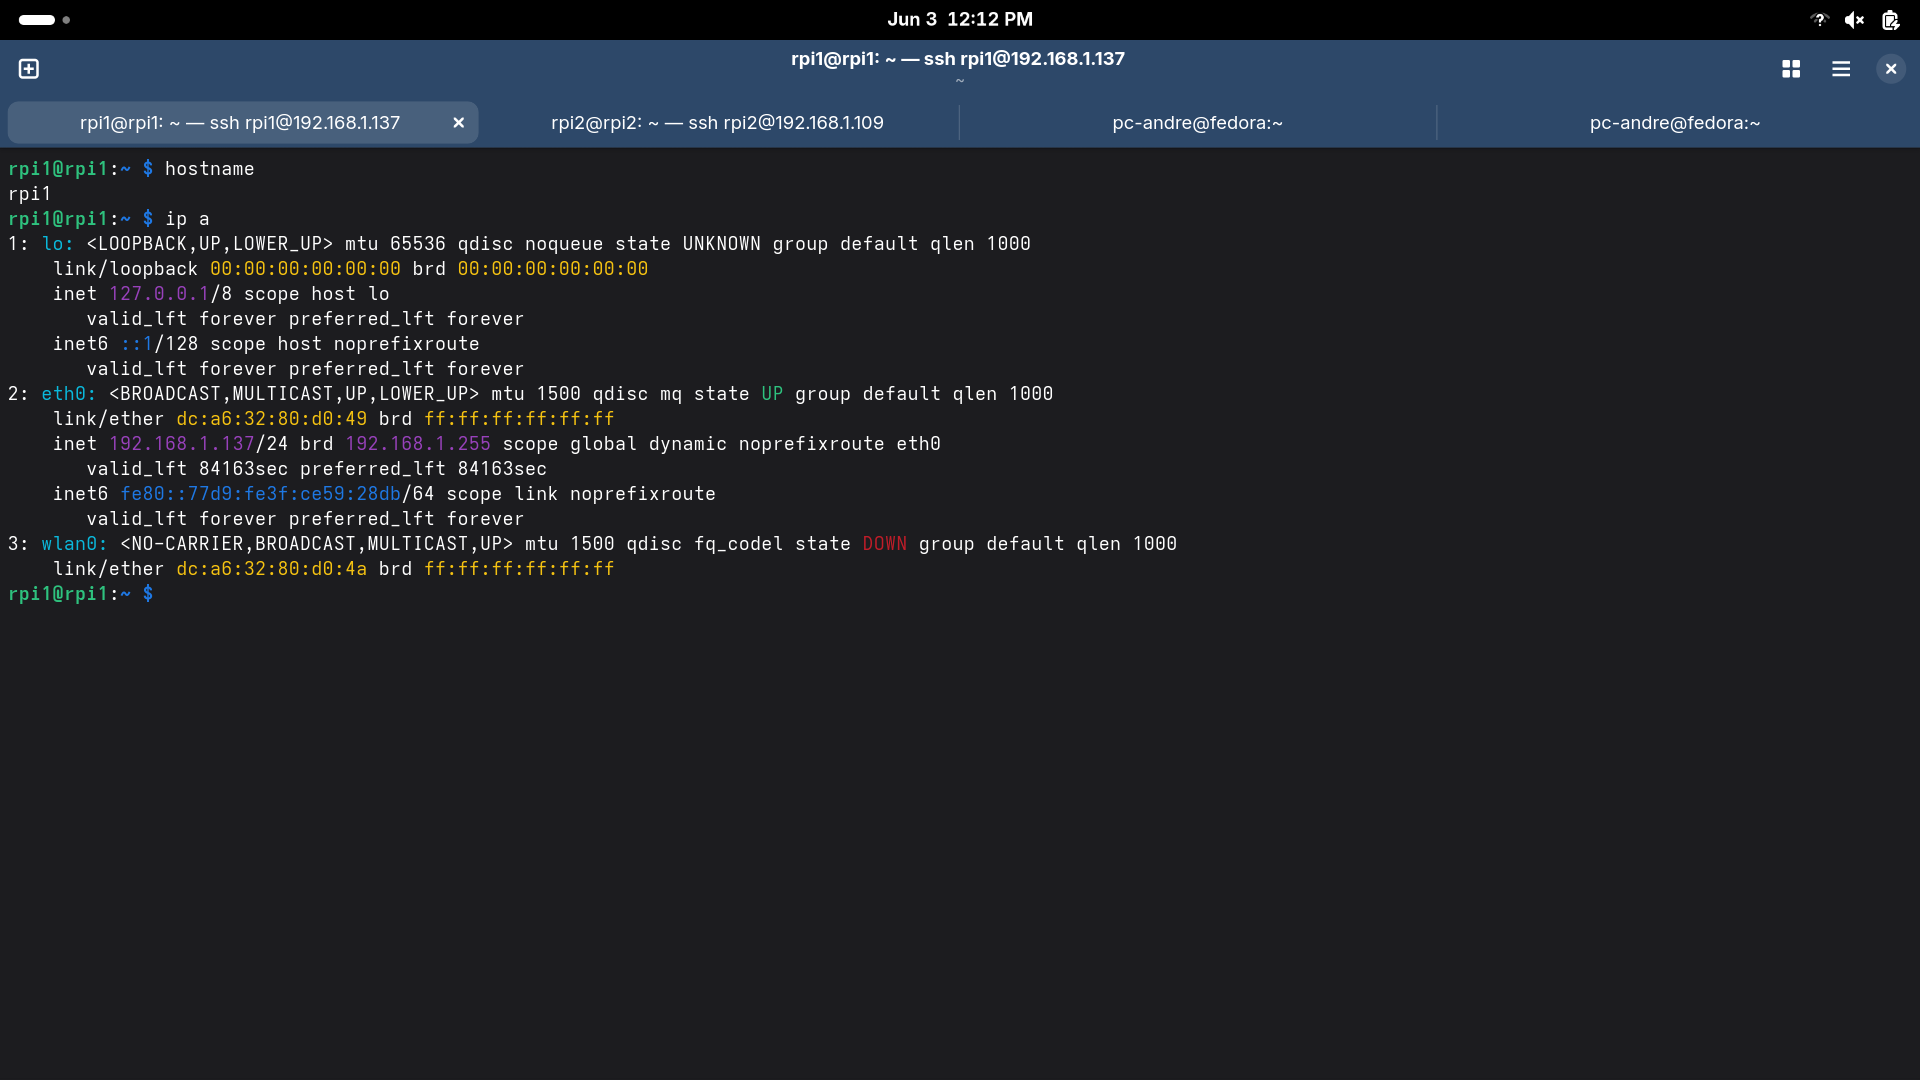
\includegraphics[width=\textwidth]{../images/A1-RPI1.png} 
        \caption*{RPI1 Interface Status}
    \end{minipage}
    \hfill
    \begin{minipage}{0.48\textwidth}
        \centering
        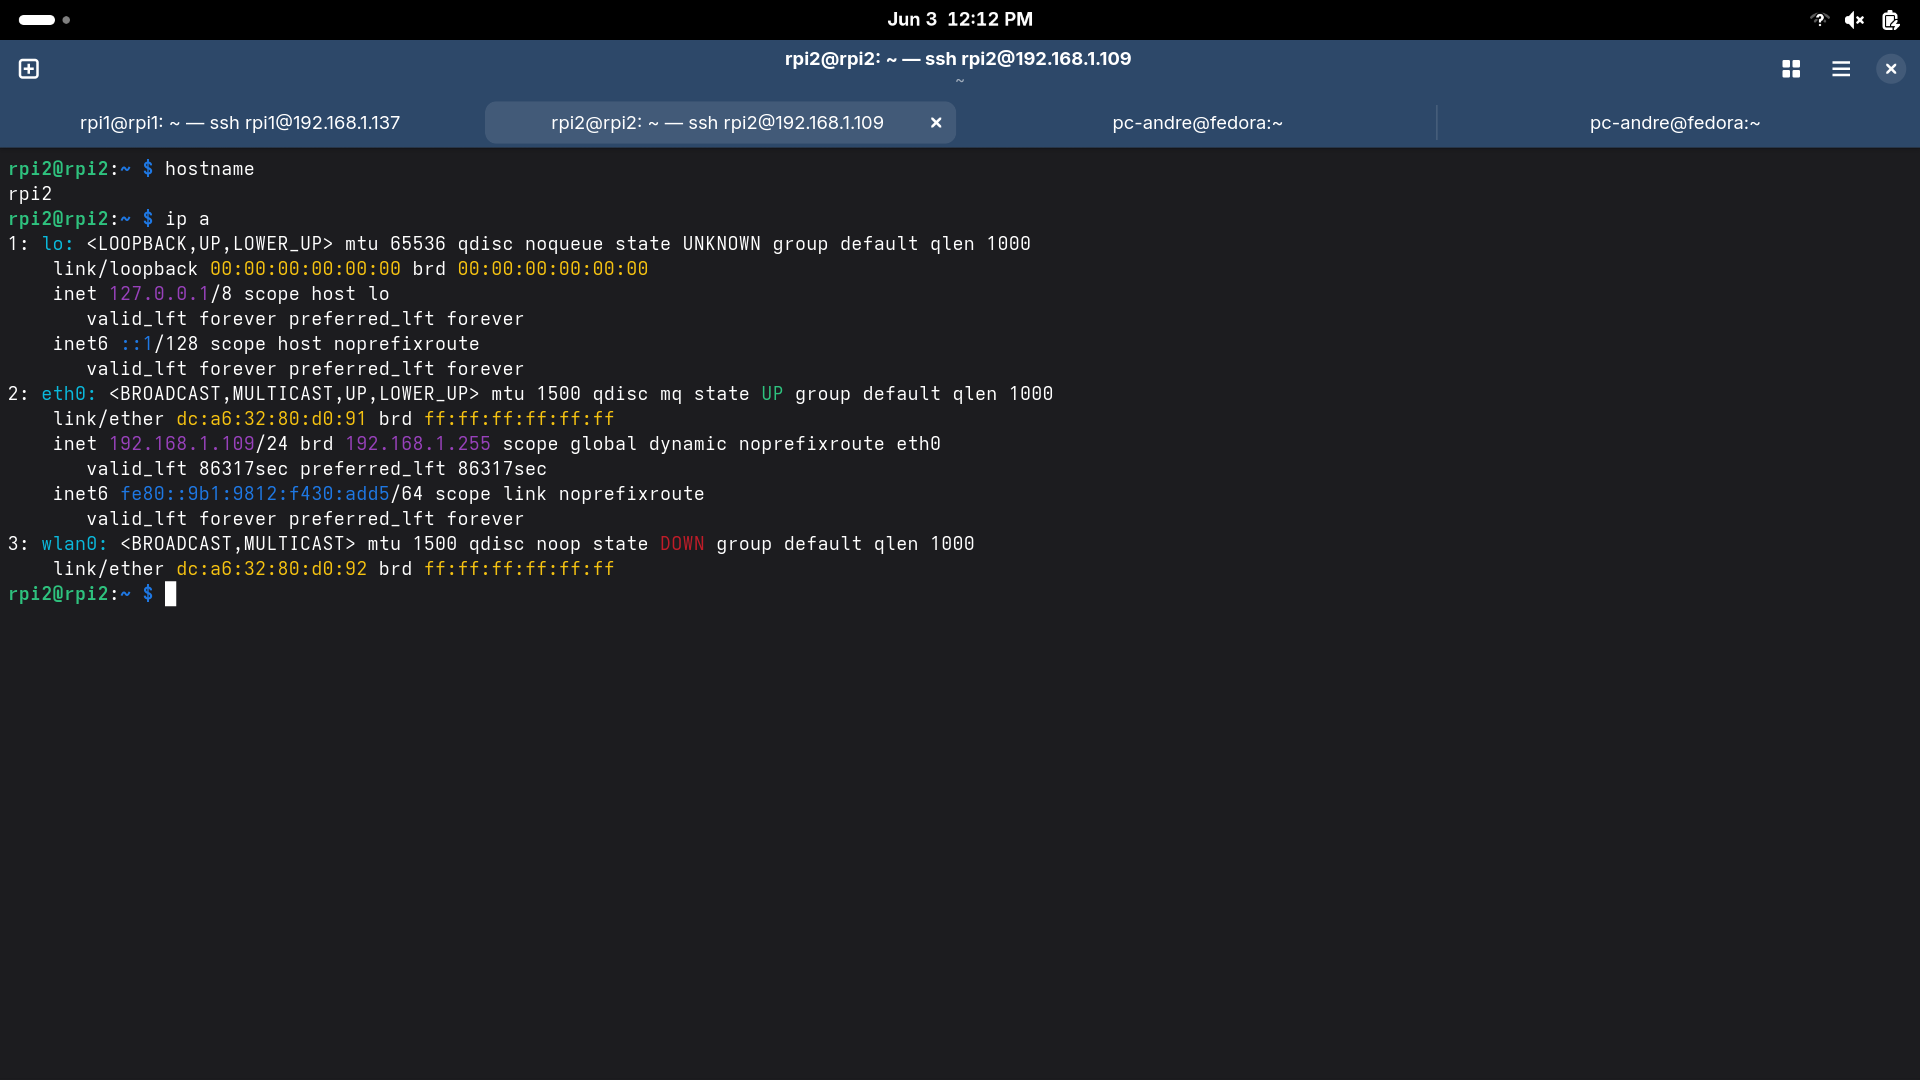
\includegraphics[width=\textwidth]{../images/A1-RPI2.png} 
        \caption*{RPI2 Interface Status}
    \end{minipage}
    \vspace{0.5cm}
    \begin{minipage}{0.8\textwidth}
        \centering
        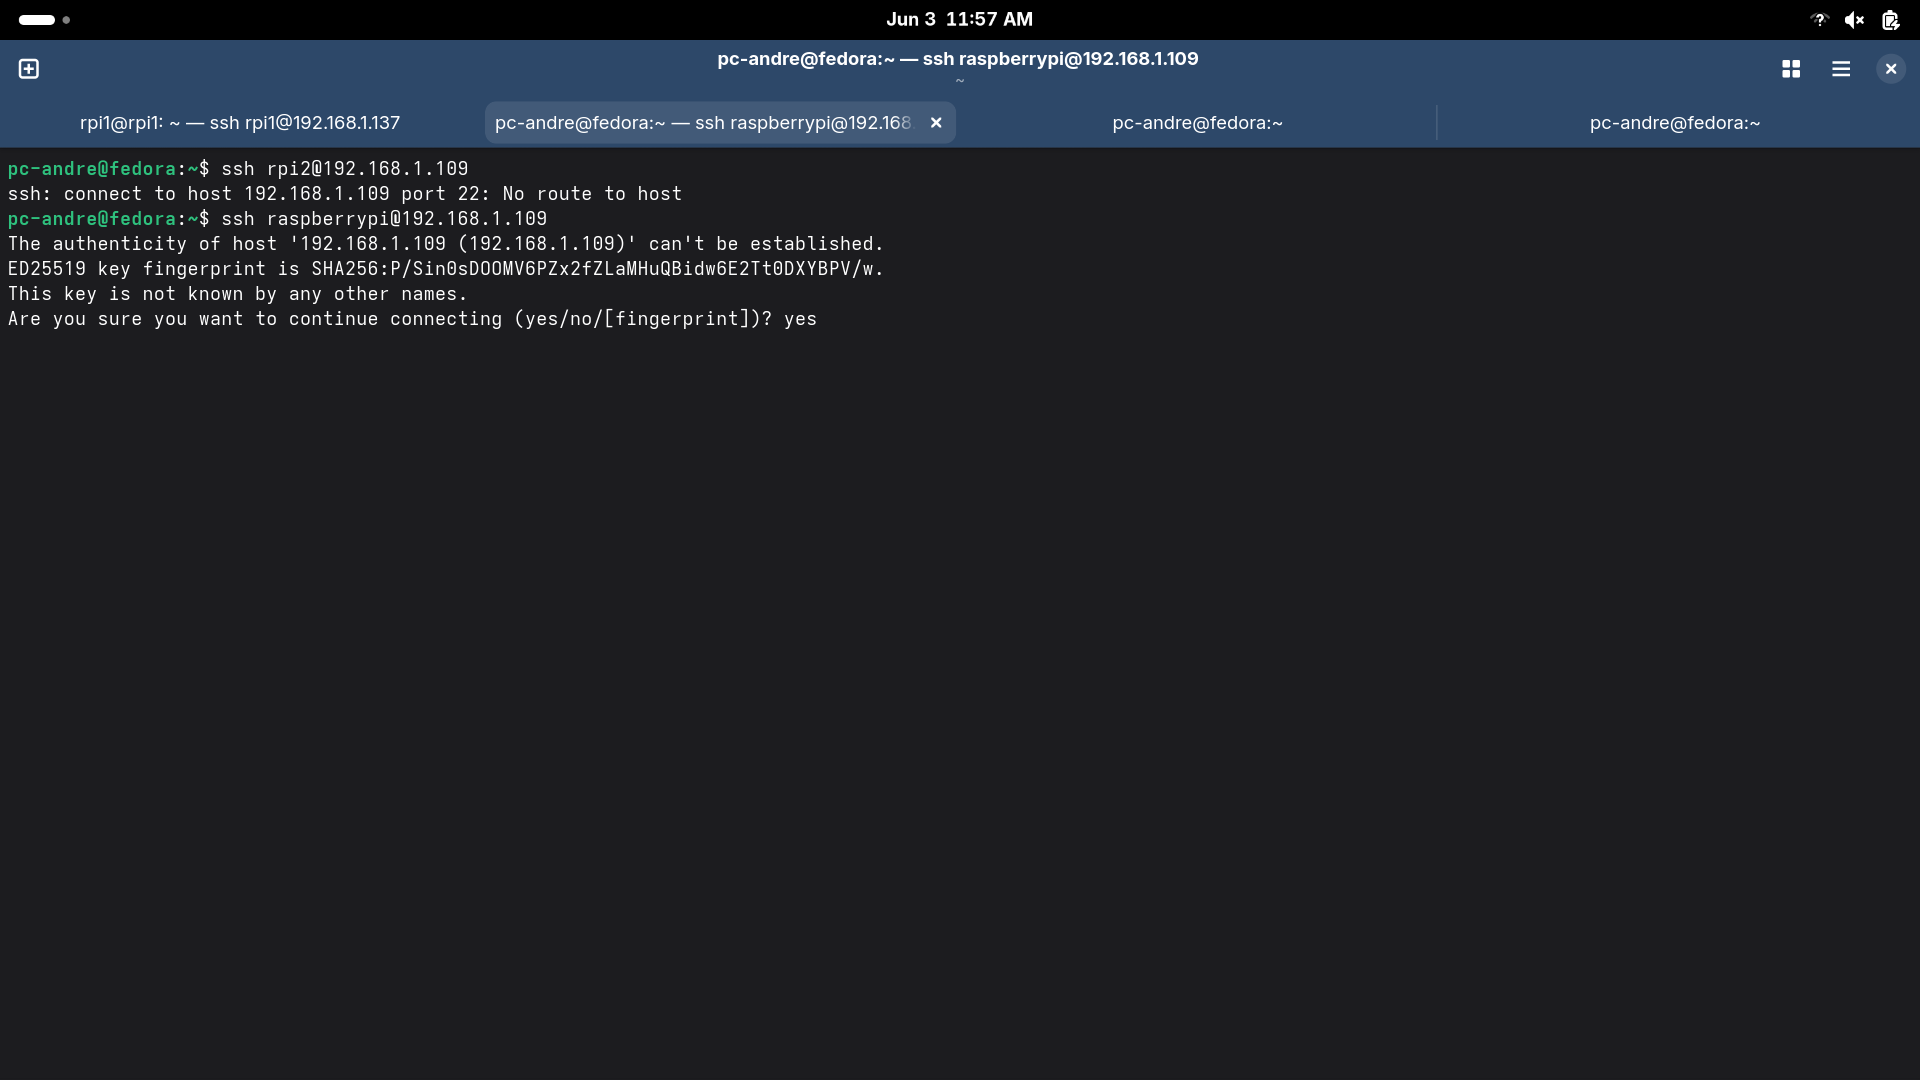
\includegraphics[width=\textwidth]{../images/SSH-RPI2.png} 
        \caption*{SSH Connection Established}
    \end{minipage}
    \caption{Verification of hostnames, interfaces, and SSH access for both Raspberry Pi units.}
    \label{fig:a1_setup}
\end{figure}

\section{Wi-Fi connection of the two RPis (A2)}
Both units were associated with the correct SSIDs provided by the assigned Wi-Fi infrastructure. The table below registers the IP addresses obtained by each RPi over the wireless interface (\texttt{wlan0}).

\begin{table}[H]
    \centering
    \caption{SSID and IP addresses for the connected Raspberry Pi units.}
    \label{tab:wifi_connection}
    \begin{tabularx}{\textwidth}{X c c}
        \toprule
        \textbf{Unit} & \textbf{SSID (2.4 GHz / 5 GHz)} & \textbf{Wireless IP Address} \\
        \midrule
        RPI1 & Recom\_AM\_PK\_2 / Recom\_AM\_PK\_5 & 192.168.1.139 \\
        RPI2 & Recom\_AM\_PK\_2 / Recom\_AM\_PK\_5 & 192.168.1.110 \\
        \bottomrule
    \end{tabularx}
\end{table}

To validate the configuration, we captured the router settings, the wireless interfaces configured, and performed initial ICMP ping tests between the nodes.

\begin{figure}[H]
    \centering
    \begin{minipage}{0.48\textwidth}
        \centering
        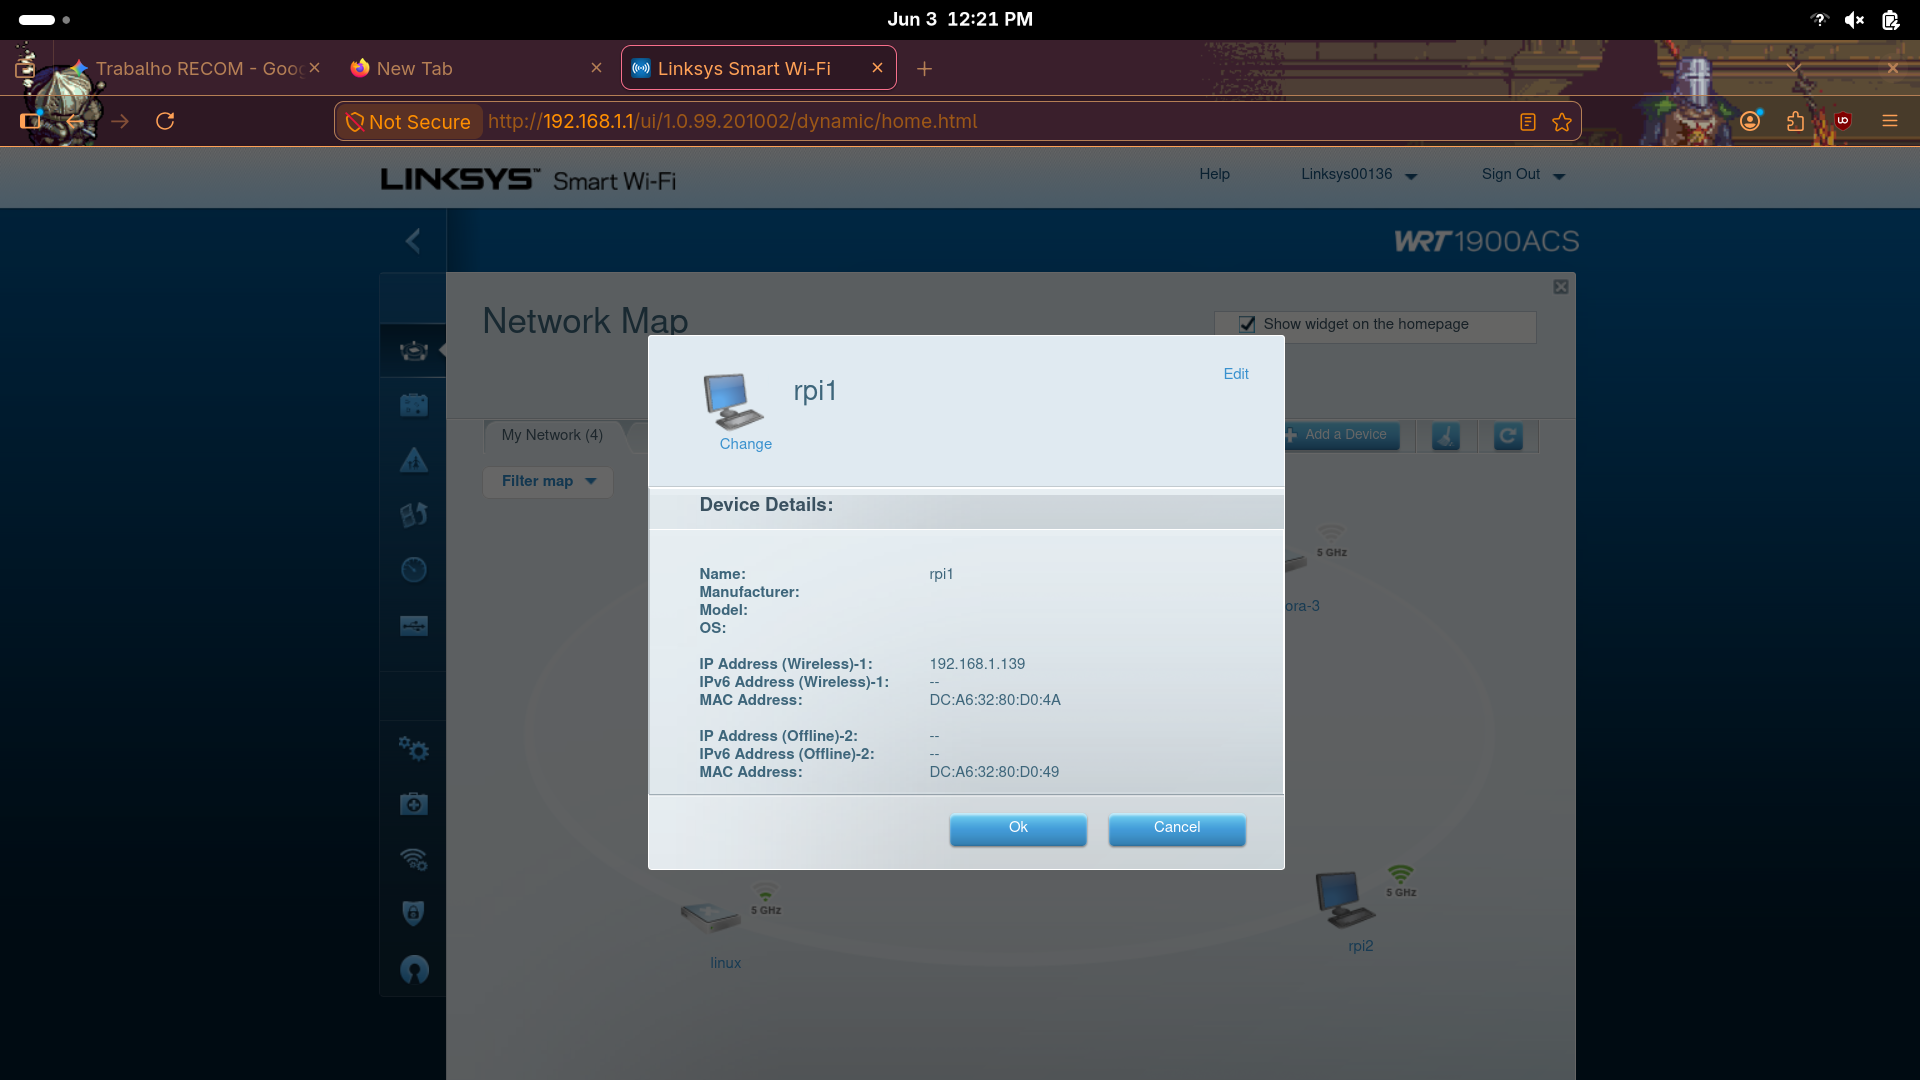
\includegraphics[width=\textwidth]{../images/RPI1-Wireless-IP.png} 
        \caption*{RPI1 Wireless IP Allocation}
    \end{minipage}
    \hfill
    \begin{minipage}{0.48\textwidth}
        \centering
        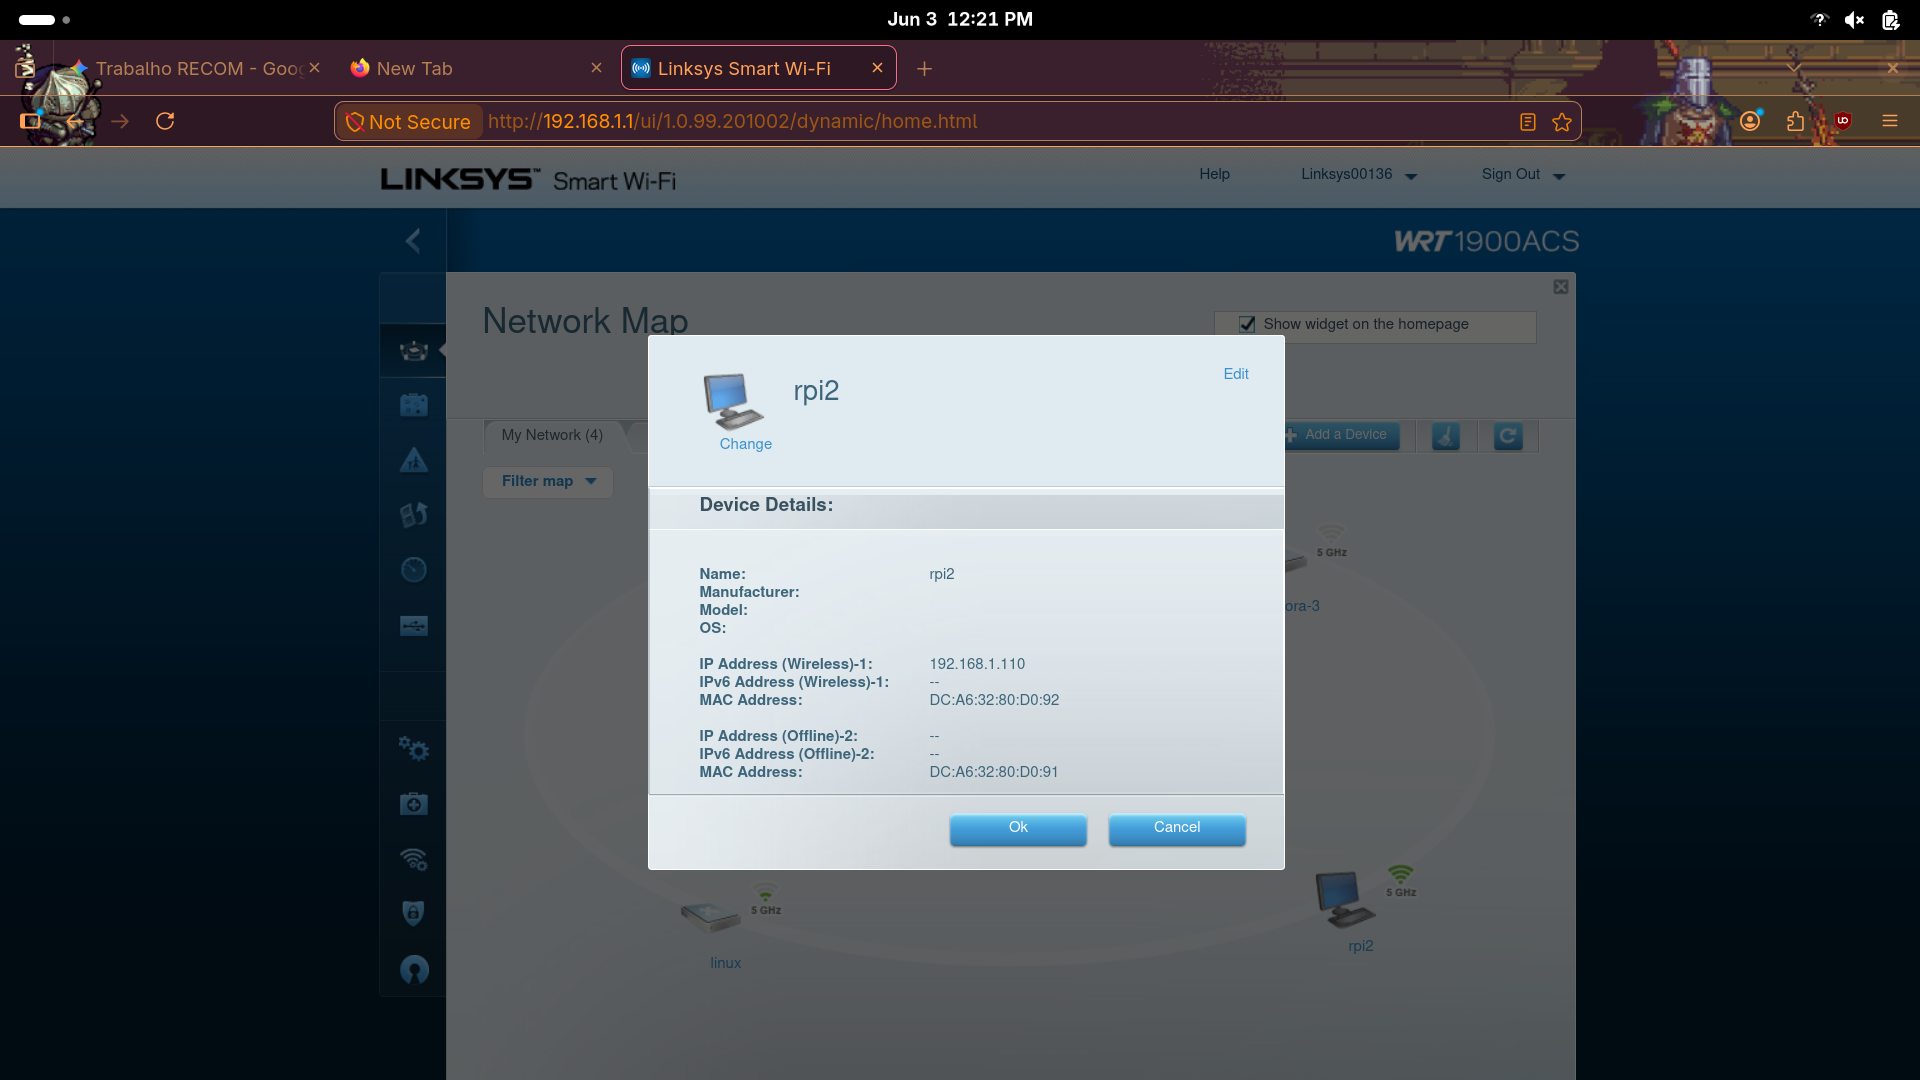
\includegraphics[width=\textwidth]{../images/RPI2-Wireless-IP.png} 
        \caption*{RPI2 Wireless IP Allocation}
    \end{minipage}
    \vspace{0.5cm}
    \begin{minipage}{0.48\textwidth}
        \centering
        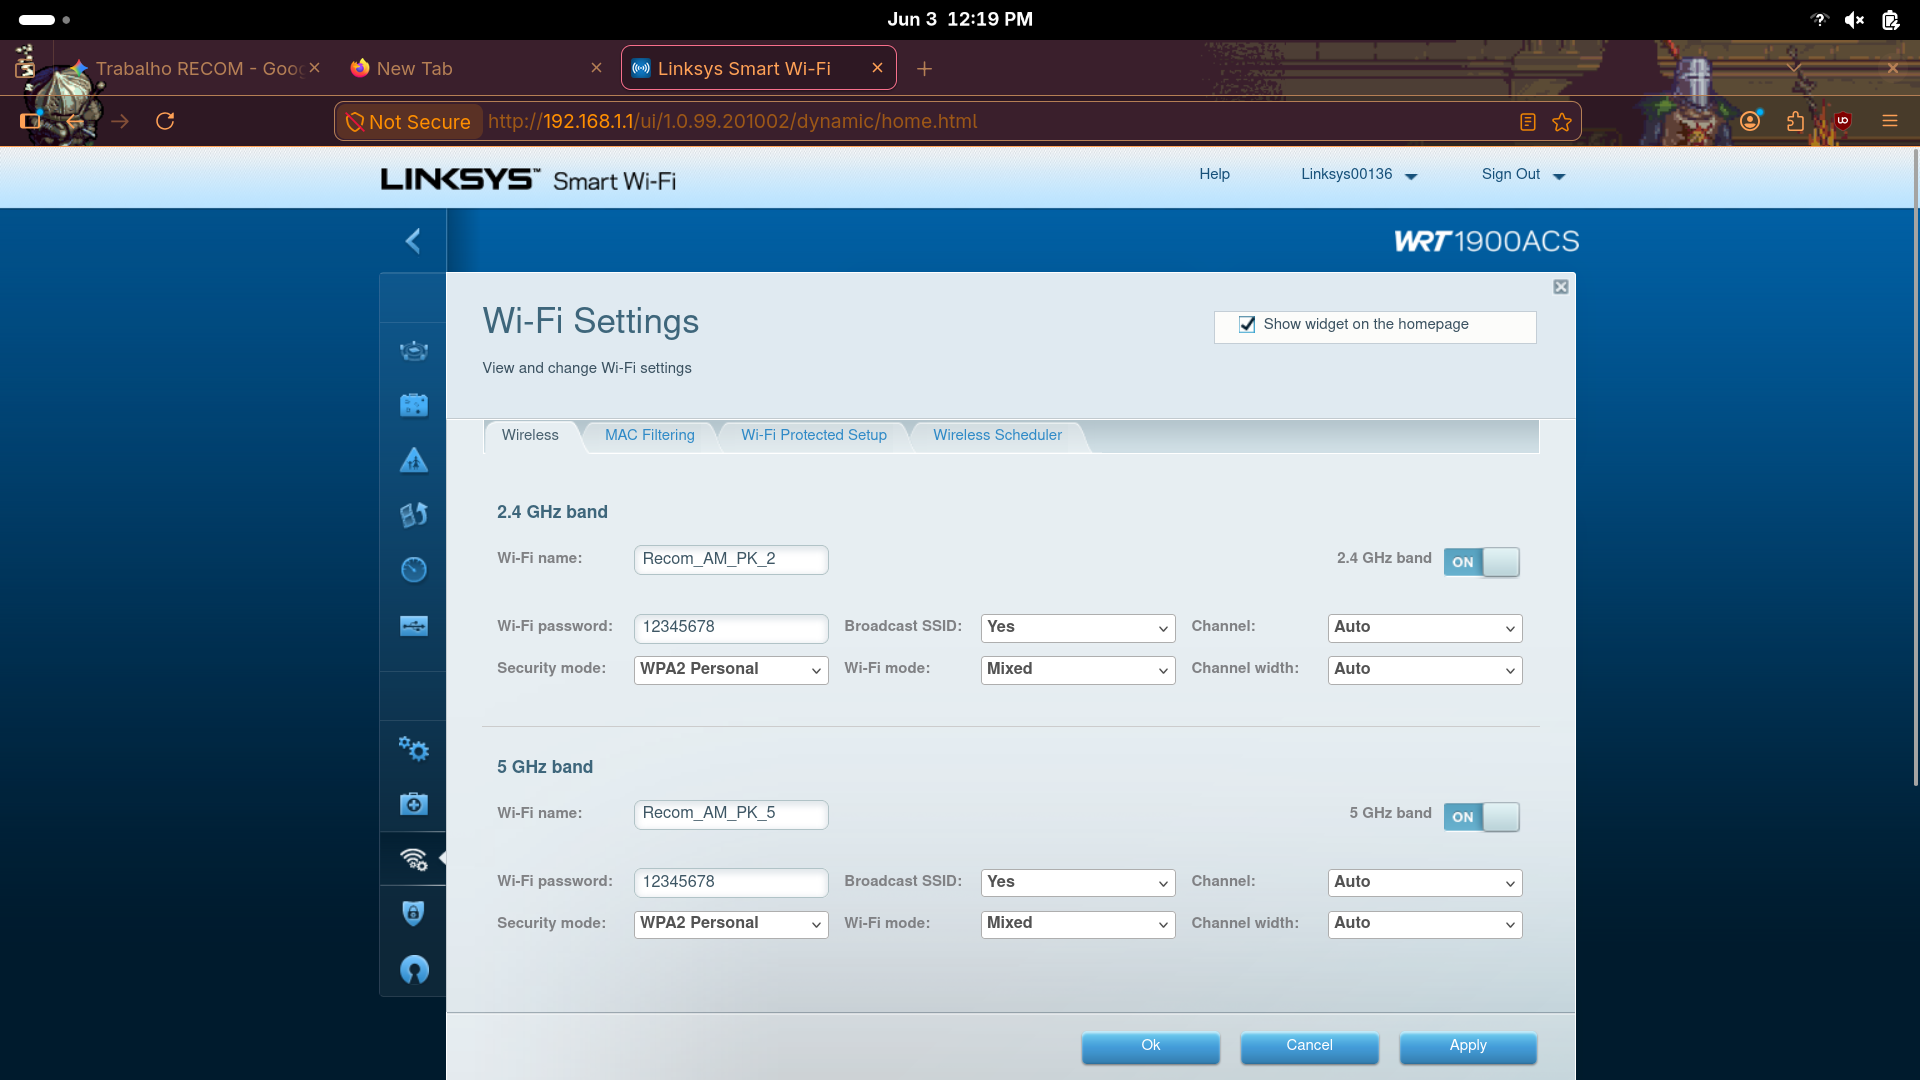
\includegraphics[width=\textwidth]{../images/Router-Settings.png} 
        \caption*{Router Wi-Fi Configurations}
    \end{minipage}
    \hfill
    \begin{minipage}{0.48\textwidth}
        \centering
        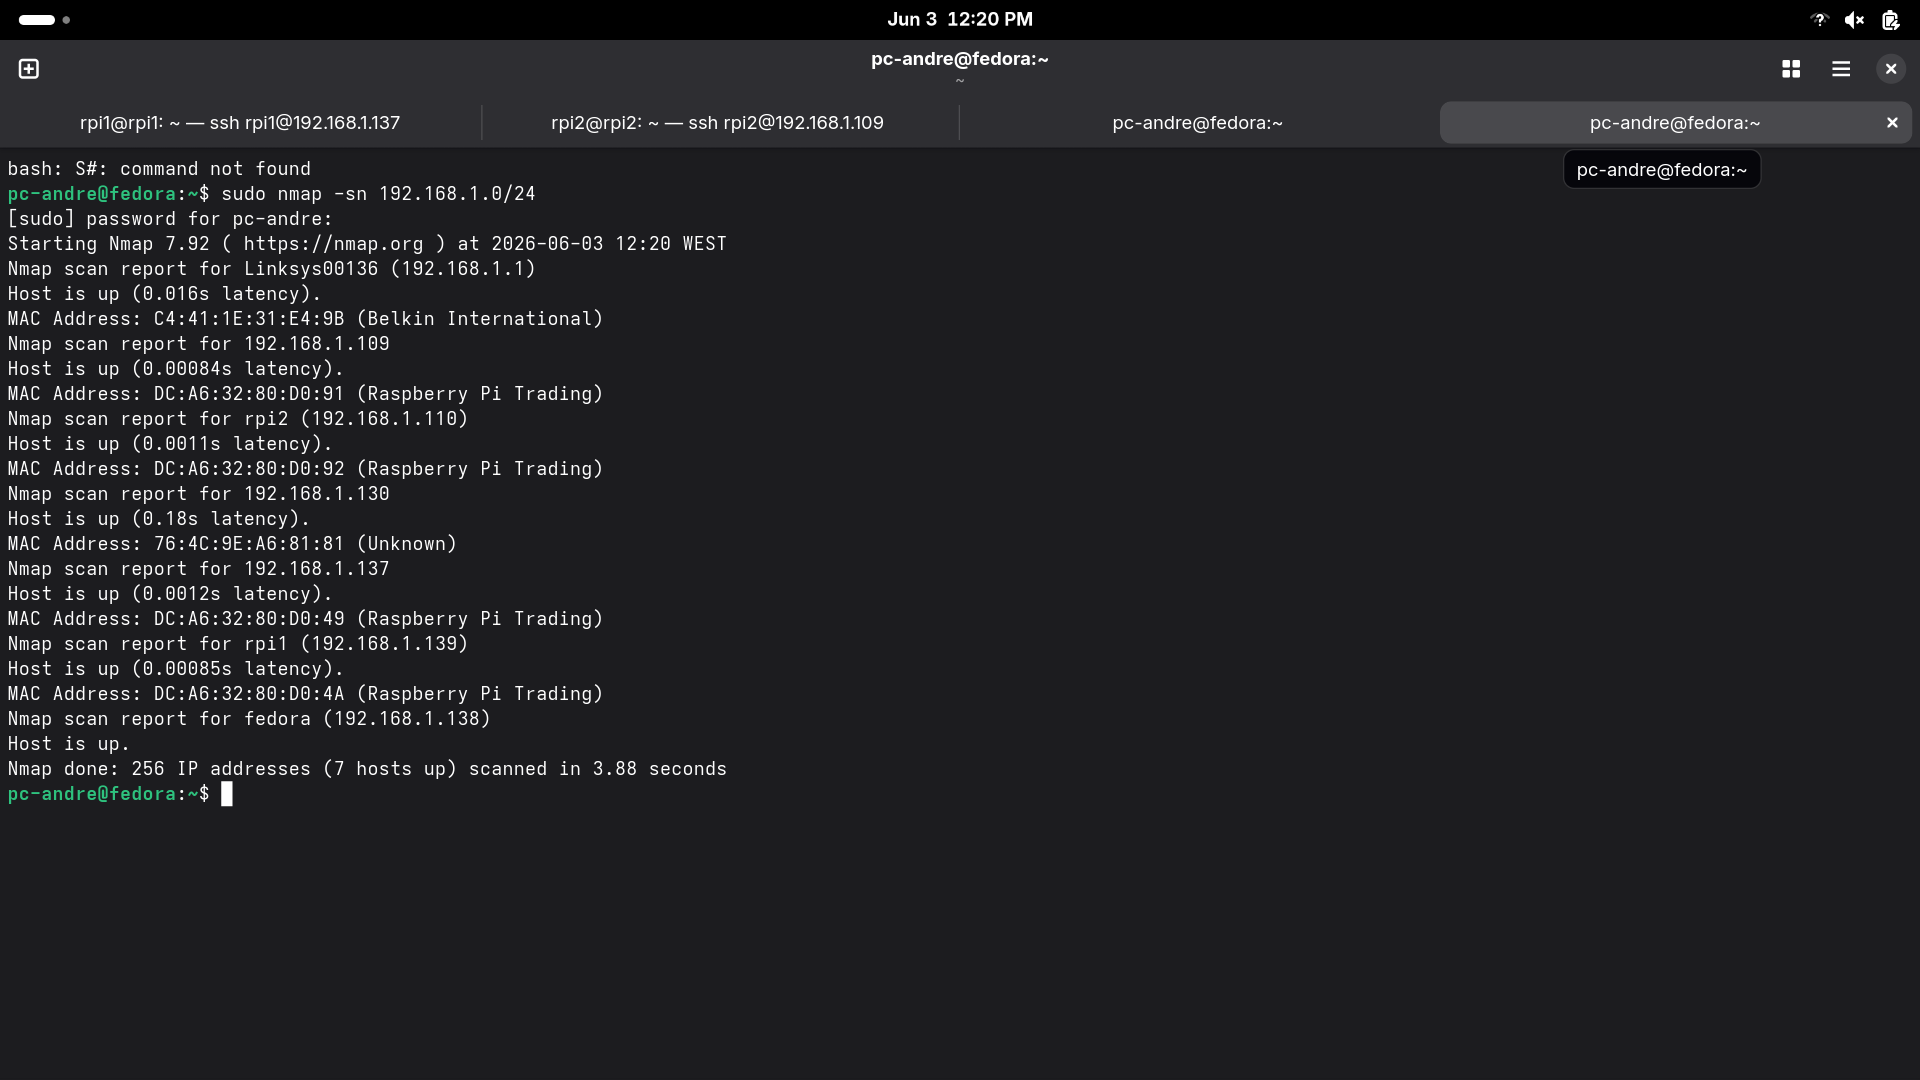
\includegraphics[width=\textwidth]{../images/Ips-da-Rede.png} 
        \caption*{Nmap Network Scan}
    \end{minipage}
    \caption{Network configuration and IP validation for the wireless infrastructure.}
    \label{fig:network_configs}
\end{figure}

\begin{figure}[H]
    \centering
    \begin{minipage}{0.48\textwidth}
        \centering
        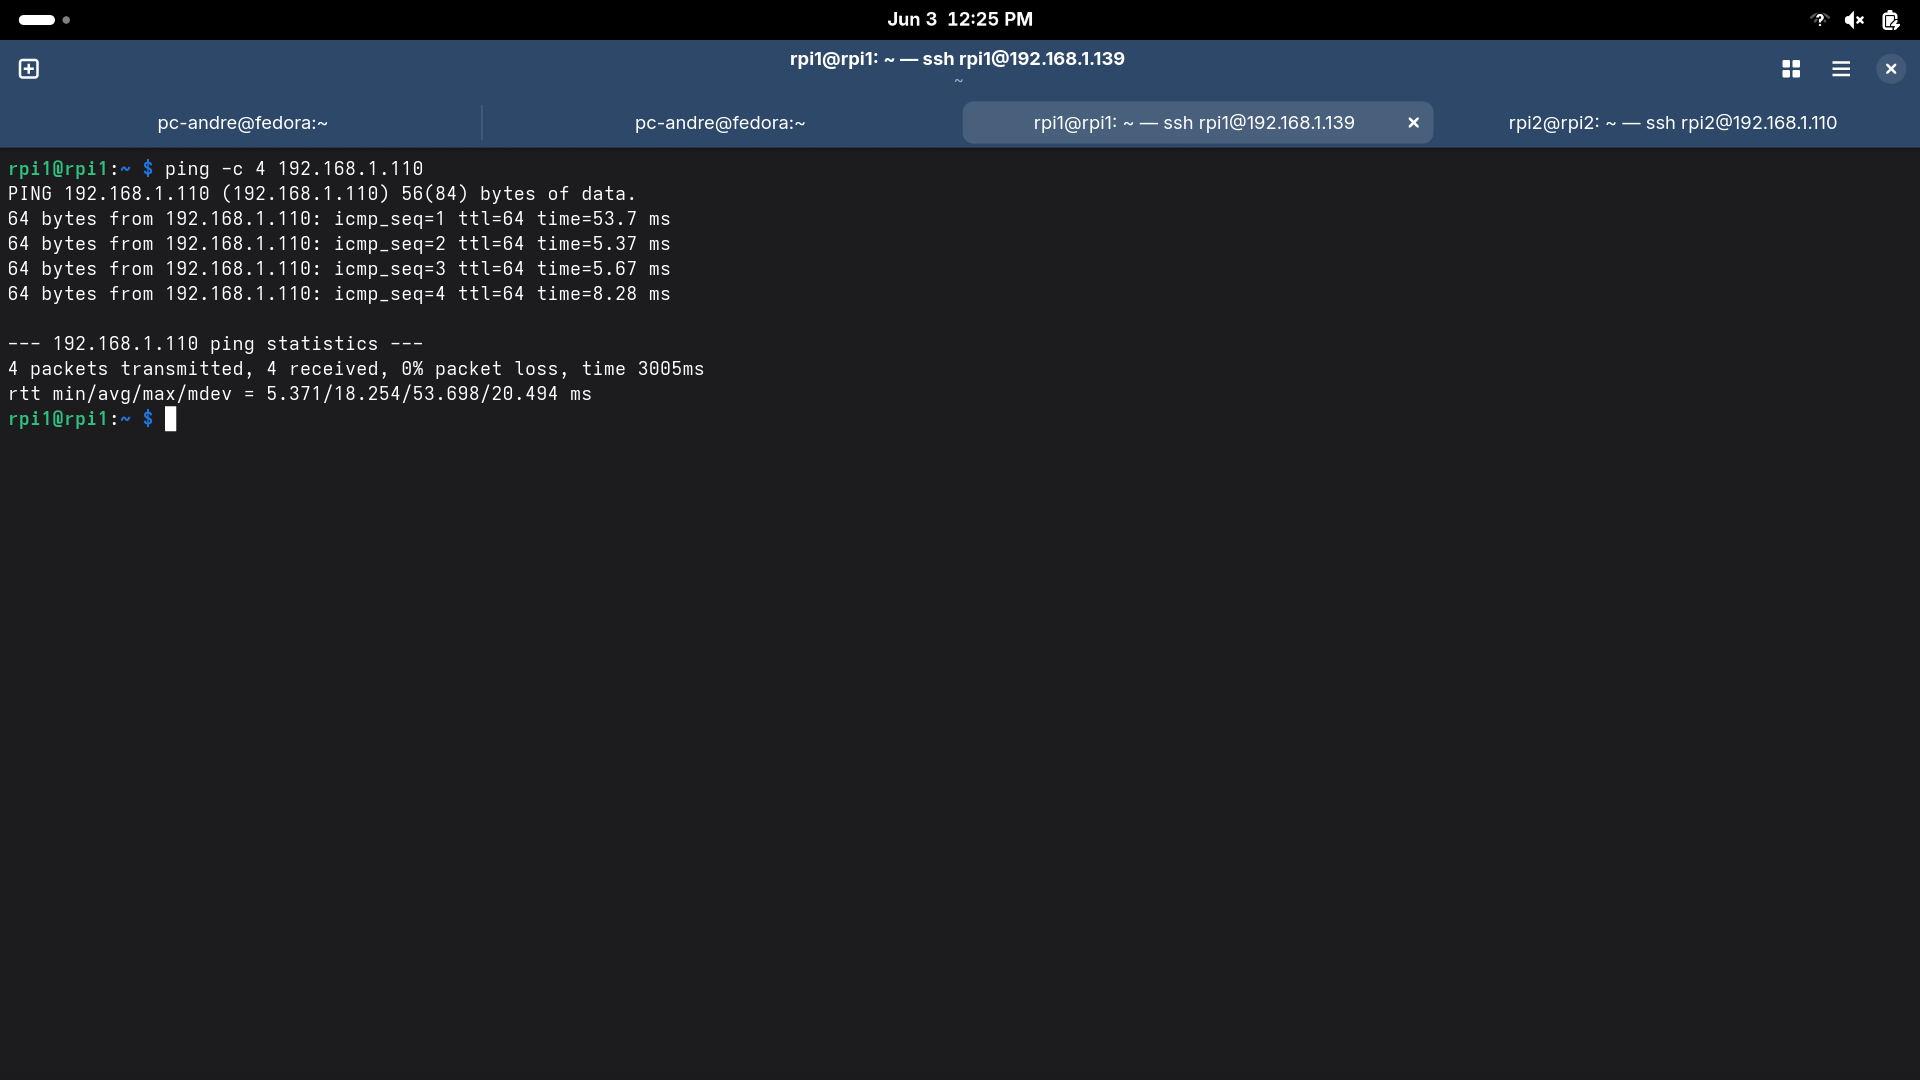
\includegraphics[width=\textwidth]{../images/A2-RPI1-Pings.png} 
        \caption*{Ping from RPI1 to RPI2}
    \end{minipage}
    \hfill
    \begin{minipage}{0.48\textwidth}
        \centering
        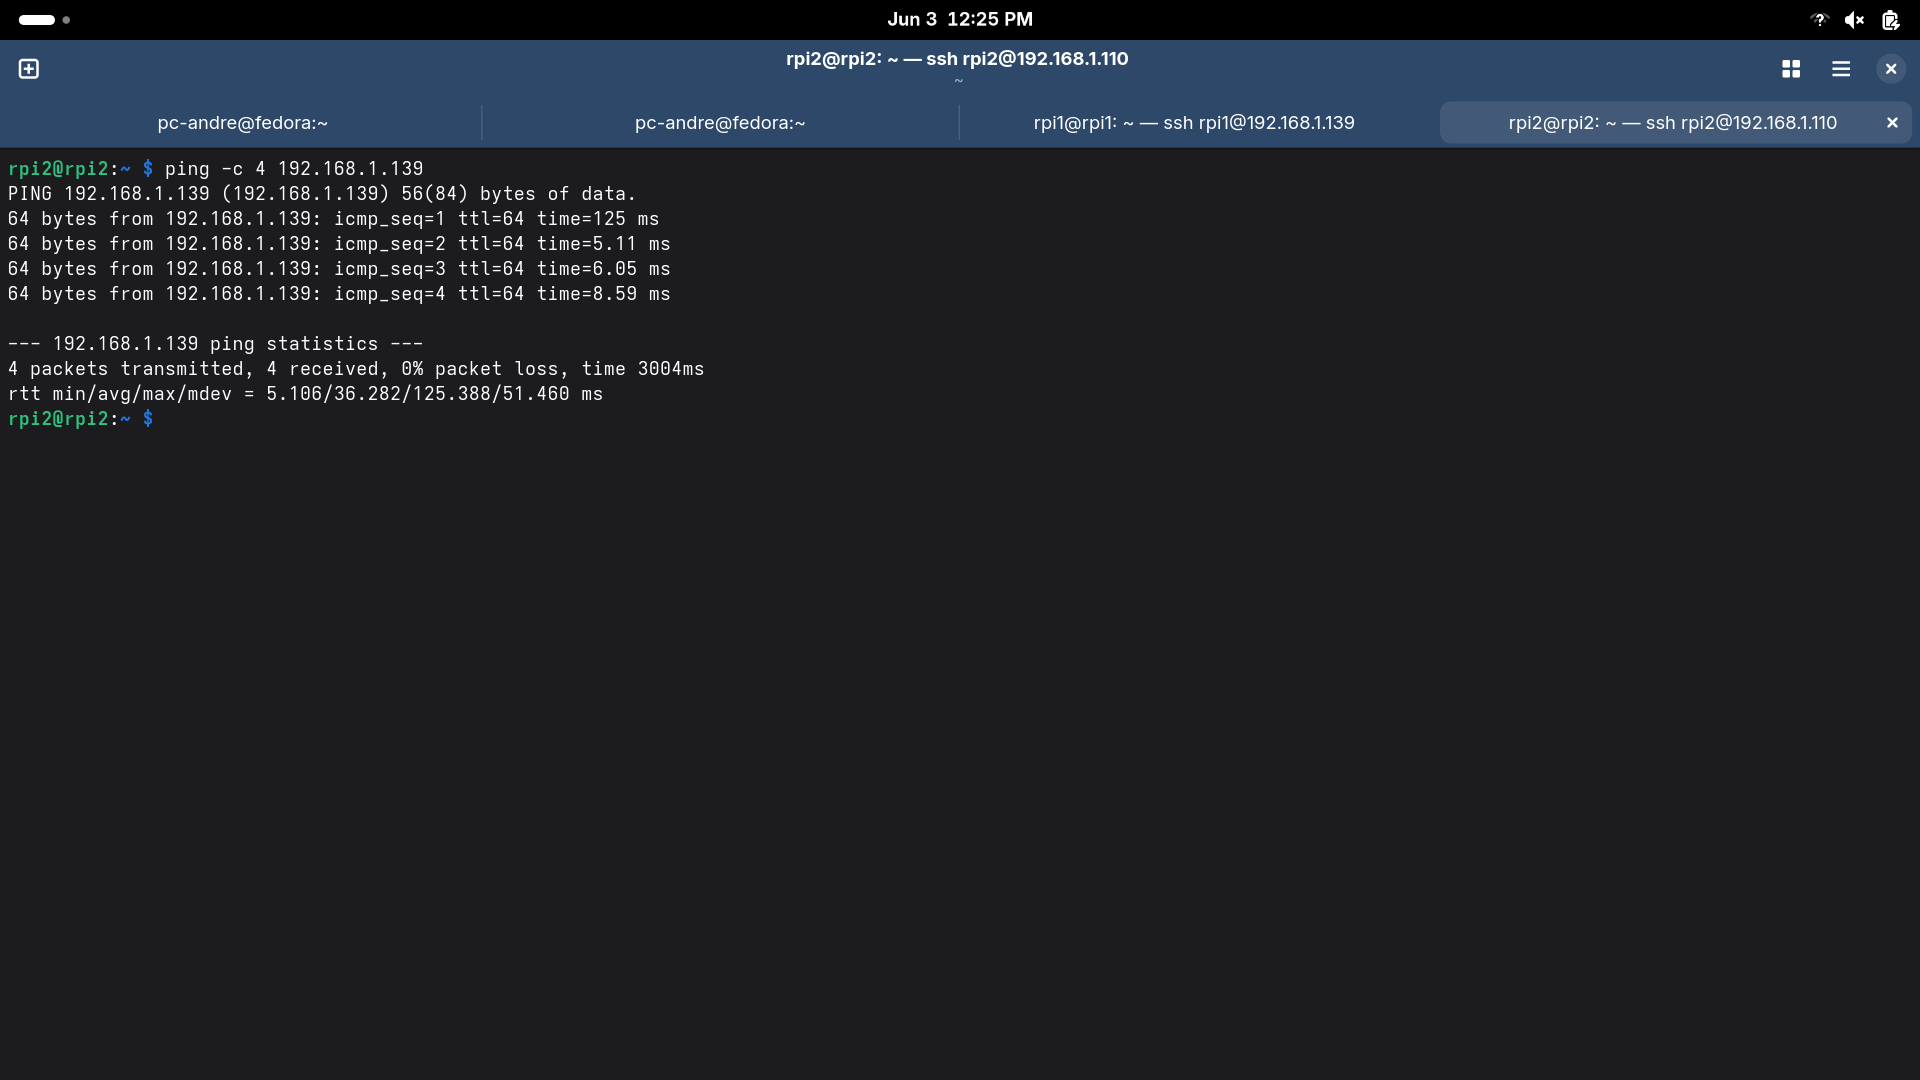
\includegraphics[width=\textwidth]{../images/A2-RPI2-Pings.png} 
        \caption*{Ping from RPI2 to RPI1}
    \end{minipage}
    \caption{Initial connectivity validation via ICMP pings between the two RPis.}
    \label{fig:initial_pings}
\end{figure}


\chapter{Part B - Wi-Fi measurements between RPI1 and RPI2}

\section{Connectivity and latency (B1)}
We executed 20 \texttt{ping} packet tests between the two RPis under a short distance with line of sight. To comprehensively analyze the network, these tests were performed independently on both the \SI{2.4}{\GHz} and \SI{5}{\GHz} bands.

\begin{table}[H]
    \centering
    \caption{Average latency and packet loss observed under short distance (Line of sight).}
    \label{tab:latency_measurements}
    \begin{tabularx}{\textwidth}{X c c}
        \toprule
        \textbf{Physical Condition} & \textbf{Average Latency (ms)} & \textbf{Packet Loss (\%)} \\
        \midrule
        Short distance (Line of sight) - \SI{2.4}{\GHz} & \SI{10.08}{\ms} & 0\% \\
        Short distance (Line of sight) - \SI{5}{\GHz} & \SI{7.64}{\ms} & 0\% \\
        \bottomrule
    \end{tabularx}
\end{table}

\textbf{Discussion:} 
As observed in the ping tests conducted at a short distance with line of sight, the \SI{5}{\GHz} band provided a lower average latency (\SI{7.64}{\ms}) compared to the \SI{2.4}{\GHz} band (\SI{10.08}{\ms}). The calculated averages reflect the bidirectional \texttt{rtt} measurements (RPI1 $\rightarrow$ RPI2 and RPI2 $\rightarrow$ RPI1). Both bands exhibited optimal reliability with 0\% packet loss across 20 packets. This behavior aligns with theoretical expectations \cite{ieee80211}, as the \SI{5}{\GHz} band typically offers less interference, reduced channel congestion, and faster data rates at close range, whereas \SI{2.4}{\GHz} is more susceptible to background noise in laboratory environments.

\begin{figure}[H]
    \centering
    \begin{minipage}{0.48\textwidth}
        \centering
        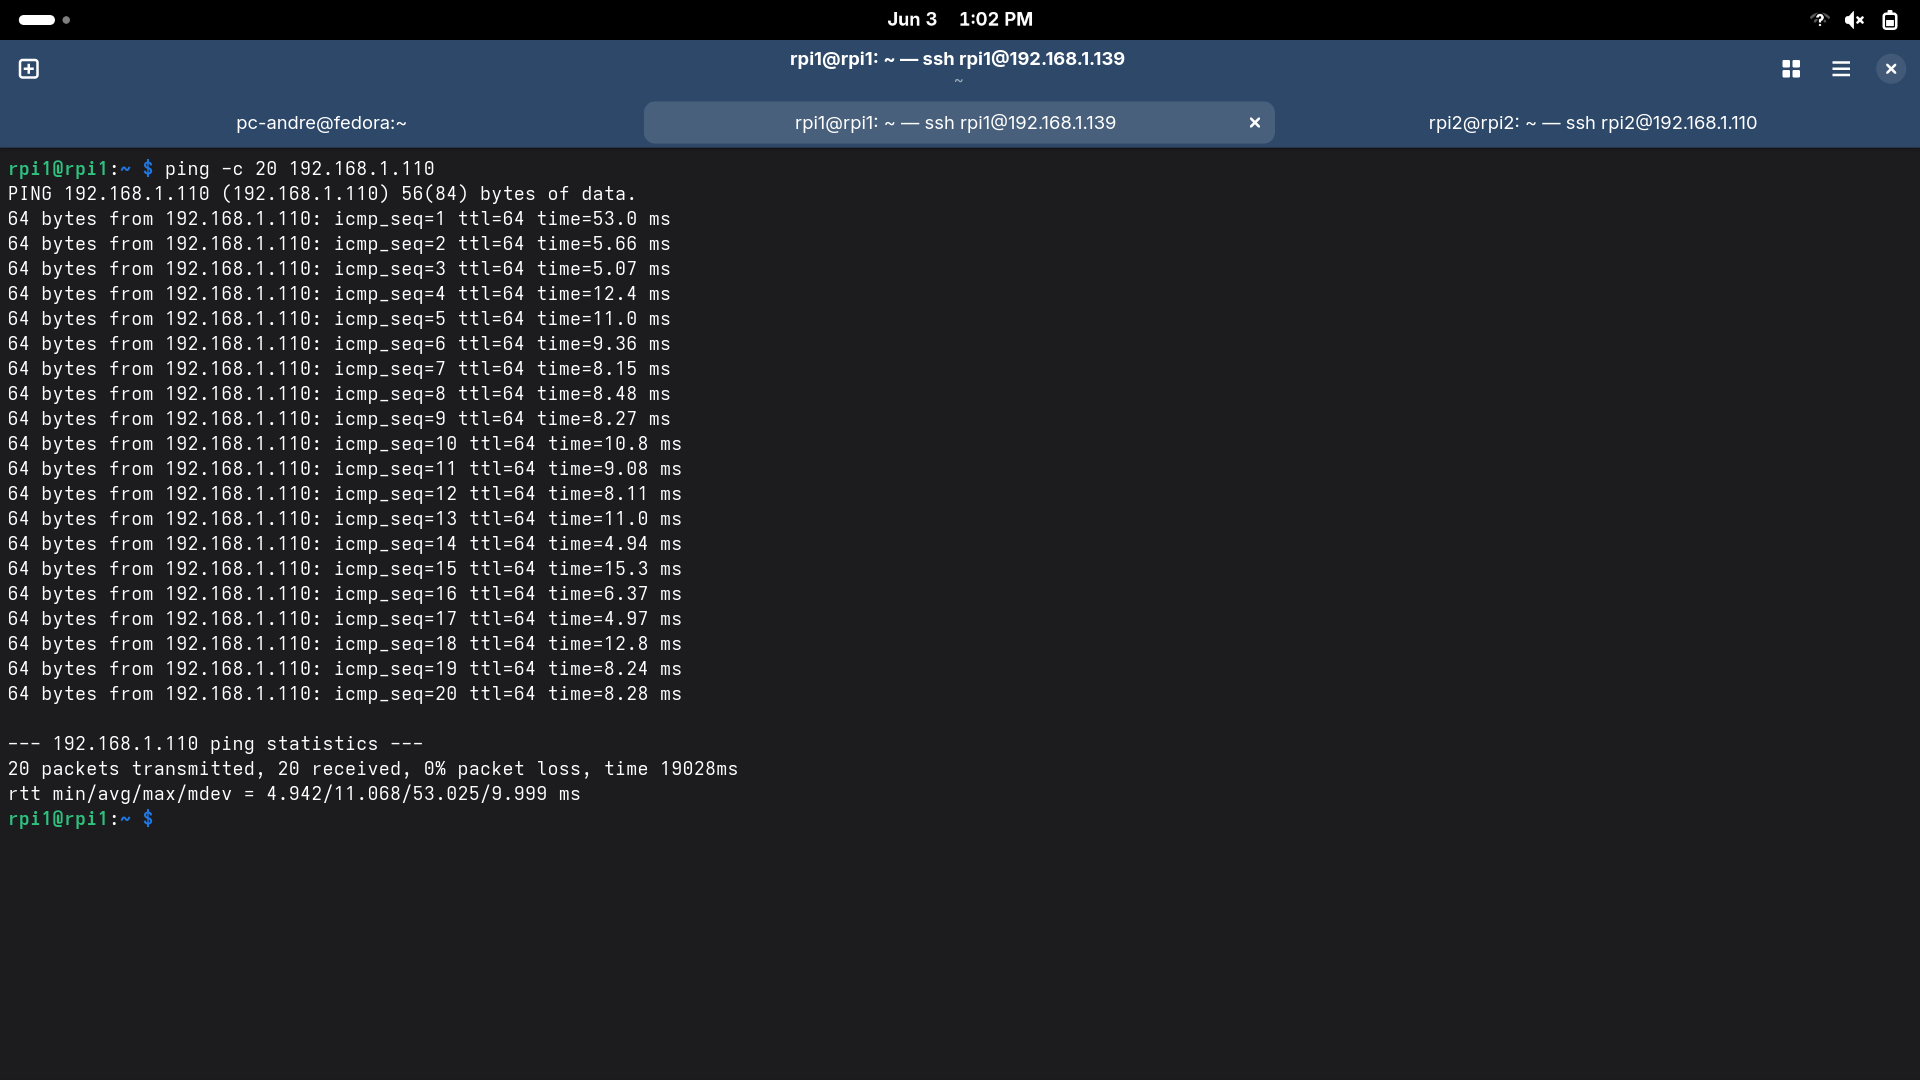
\includegraphics[width=\textwidth]{../images/rpi1-b1-perto-2.4GHZ.png} 
        \caption*{RPI1 Ping (\SI{2.4}{\GHz})}
    \end{minipage}
    \hfill
    \begin{minipage}{0.48\textwidth}
        \centering
        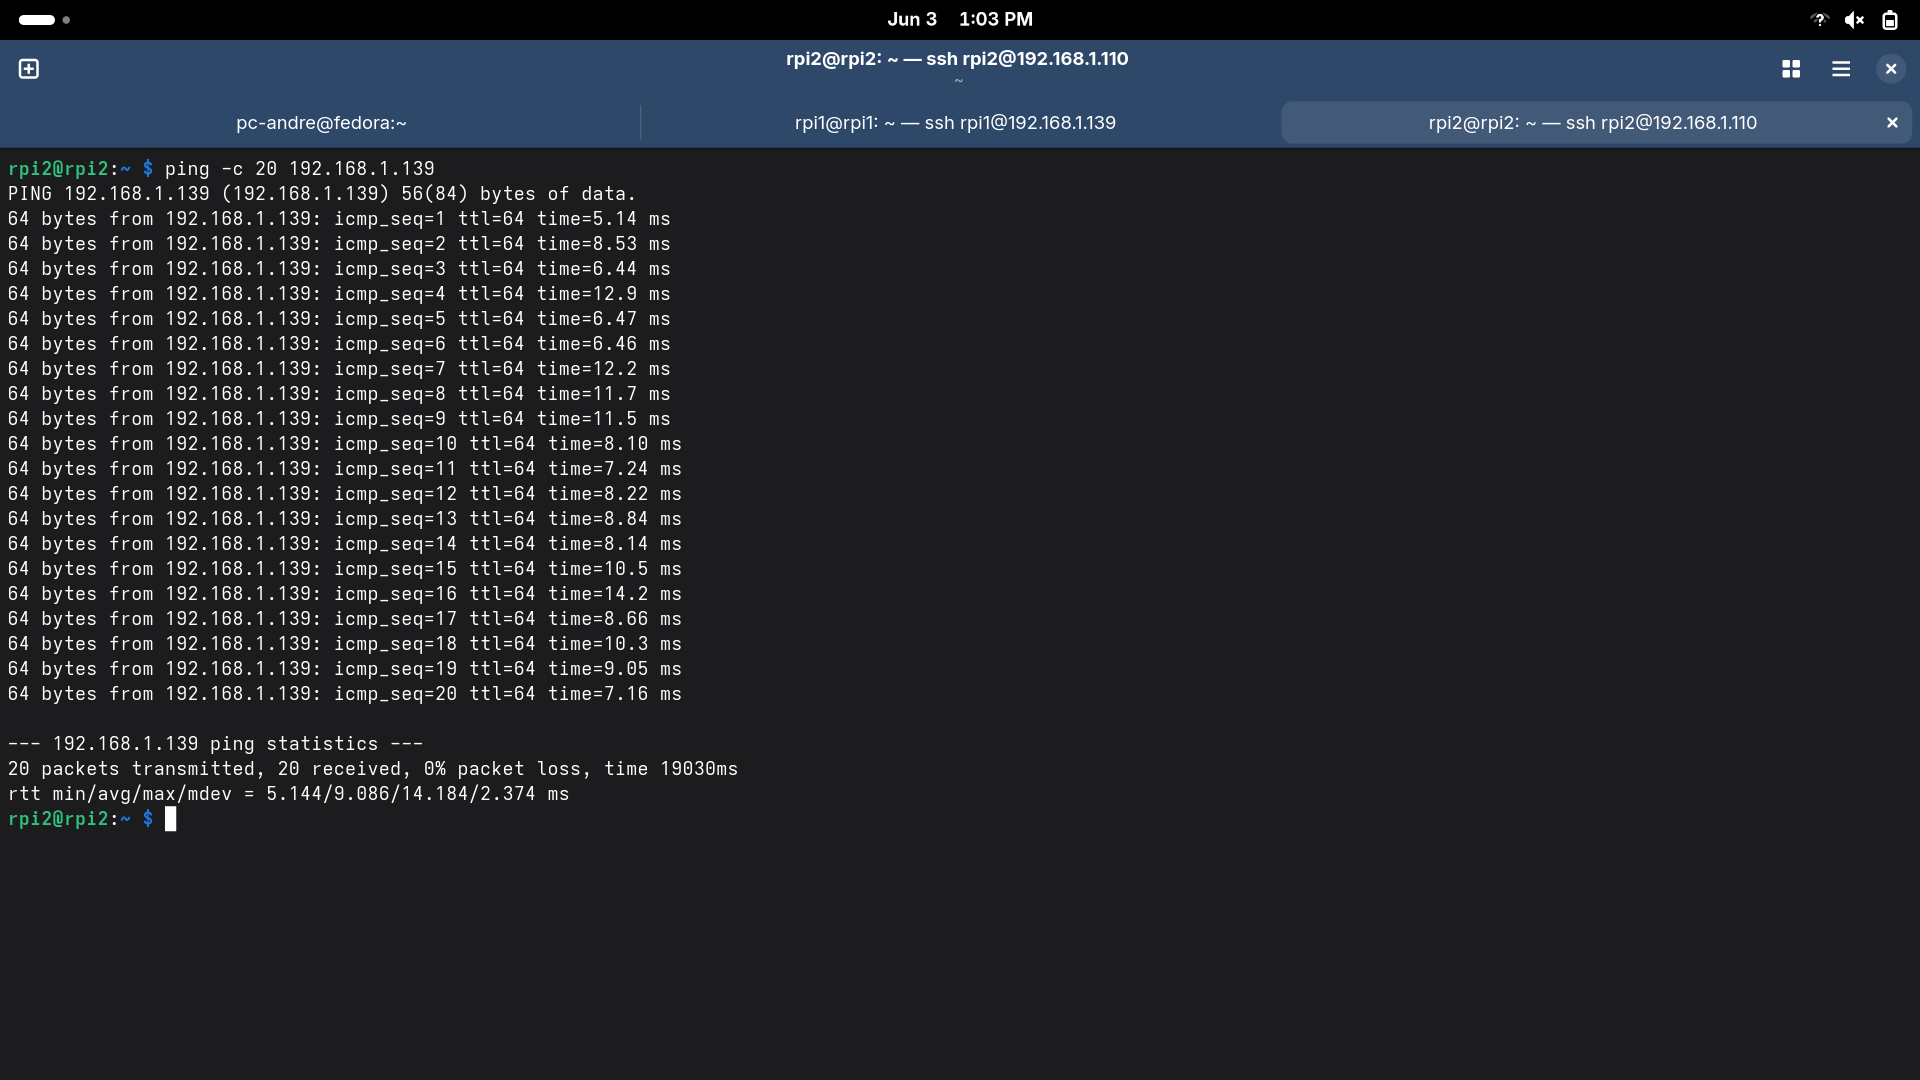
\includegraphics[width=\textwidth]{../images/rpi2-b1-perto-2.4GHZ.png} 
        \caption*{RPI2 Ping (\SI{2.4}{\GHz})}
    \end{minipage}
    \vspace{0.5cm}
    \begin{minipage}{0.48\textwidth}
        \centering
        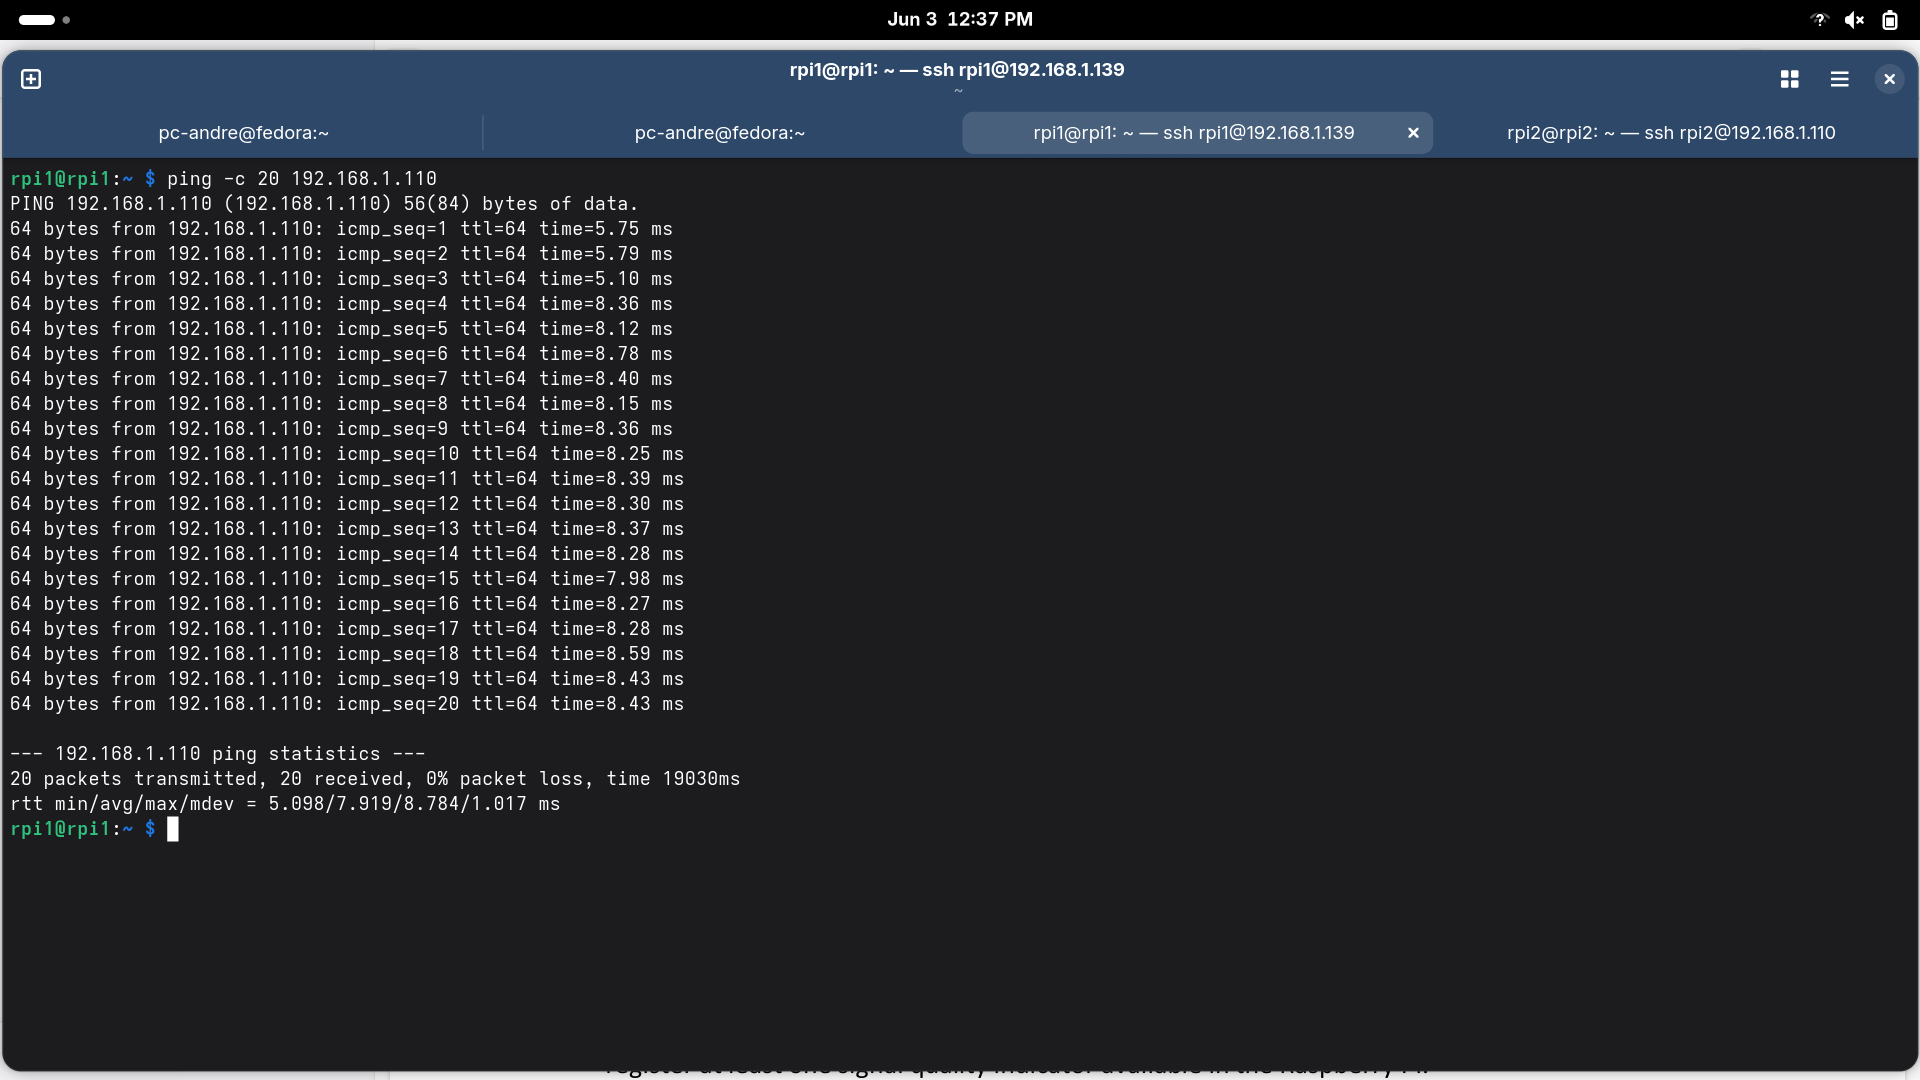
\includegraphics[width=\textwidth]{../images/rpi1-b1-perto-5GHZ.png} 
        \caption*{RPI1 Ping (\SI{5}{\GHz})}
    \end{minipage}
    \hfill
    \begin{minipage}{0.48\textwidth}
        \centering
        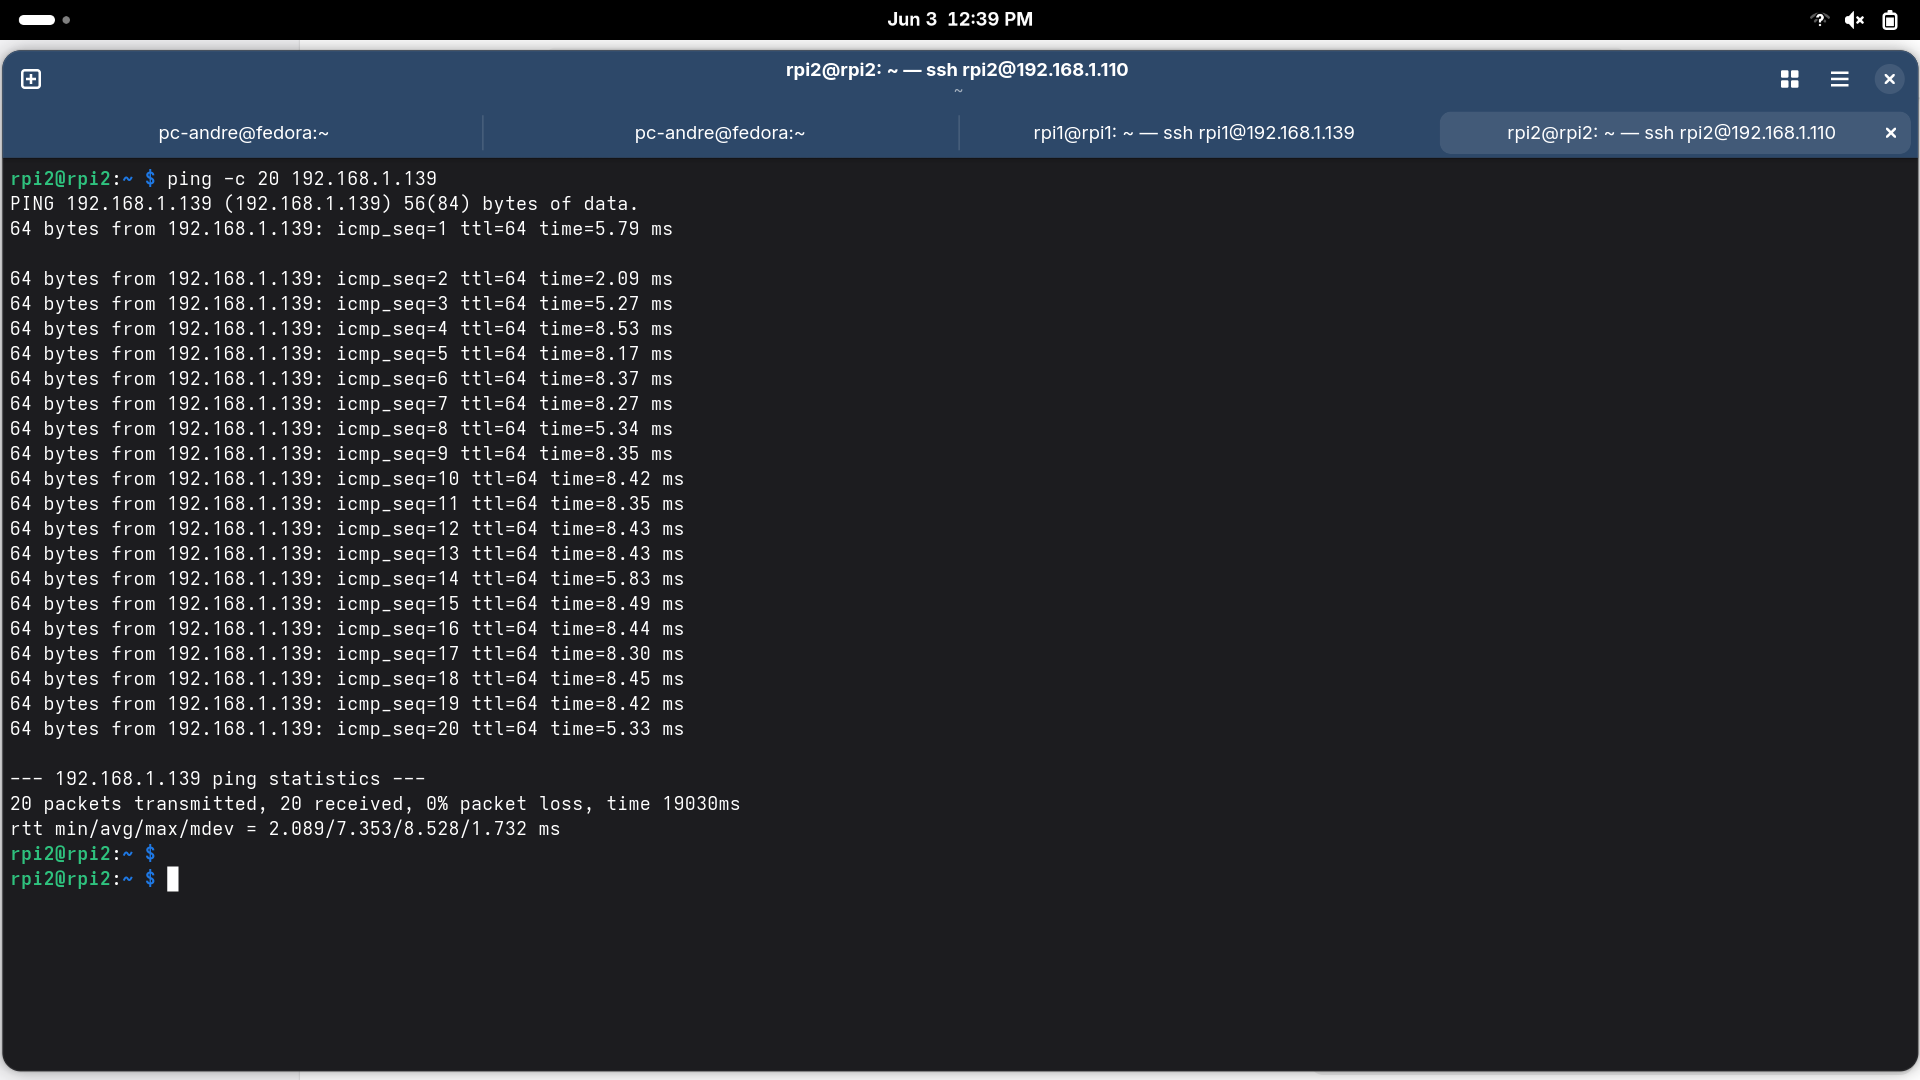
\includegraphics[width=\textwidth]{../images/rpi2-b1-perto-5GHZ.png} 
        \caption*{RPI2 Ping (\SI{5}{\GHz})}
    \end{minipage}
    \caption{Latency measurements via ping (20 packets) for both frequency bands.}
    \label{fig:latency_captures}
\end{figure}

\chapter{Conclusion}
The initial setup successfully established a wireless network between two Raspberry Pi units using a Linksys router, configuring both \SI{2.4}{\GHz} and \SI{5}{\GHz} bands. Remote access via SSH was proven to be stable, facilitating headless management. 

In the connectivity tests, the \SI{5}{\GHz} band demonstrated superior performance at short distances, presenting lower latency and excellent stability. Further sections of this laboratory will build upon this functional baseline.

\printbibliography

\end{document}